\documentclass[reprint, superscriptaddress, amsmath, amssymb, aps, prl floatfix]{revtex4-2}
\usepackage{graphicx} % Required for inserting images
\usepackage{bm}% bold math

\usepackage[caption=false]{subfig}
\usepackage[usenames,dvipsnames]{color}
\usepackage{xcolor}
\usepackage{orcidlink}
\usepackage{booktabs}

\newcommand{\ICTS}{International Centre for Theoretical Sciences,
    Tata Institute of Fundamental Research, Bangalore 560089, India}
\newcommand{\IITM}{Department of Physics, Indian Institute of Technology Madras, Chennai 600036, India}
\newcommand{\CSGC}{Centre for Strings, Gravitation and Cosmology, Department of Physics, Indian Institute of Technology Madras, Chennai 600036, India}
\newcommand{\AEI}{Max Planck Institute for Gravitational Physics (Albert Einstein Institute), Am M{\"u}hlenberg 1, 14476 Potsdam, Germany}
\newcommand{\UMass}{Department of Mathematics, Center for Scientific Computing and Data Science Research, University of Massachusetts, Dartmouth, MA 02747, USA
}

\newcommand{\param}{\bm{\theta}}
\newcommand{\eref}{e_{\rm{ref}}}
\newcommand{\lref}{l_{\rm{ref}}}

\newcommand{\esigmahm}{\texttt{ESIGMAHM}}
\newcommand{\inspiralesigma}{\texttt{InspiralESIGMA}}
\newcommand{\imresigma}{\texttt{IMRESIGMA}}
\newcommand{\nrsur}{\texttt{NRSur7dq4}}

\begin{document}

\title{Chase Orbits, not Time: A Scalable Paradigm for Long-Duration Eccentric Gravitational-Wave Surrogates}

\author{Akash Maurya \orcidlink{0009-0006-9399-9168}}\email{akash.maurya@icts.res.in}\affiliation{\ICTS}
\author{Prayush Kumar \orcidlink{0000-0001-5523-4603}}\email{prayush@icts.res.in}\affiliation{\ICTS}
\author{Scott E. Field \orcidlink{0000-0002-6037-3277}}\affiliation{\UMass}
\author{Chandra Kant Mishra \orcidlink{0000-0002-8115-8728}}\affiliation{\CSGC}\affiliation{\IITM}
\author{Peter James Nee \orcidlink{0000-0002-2362-5420}}\affiliation{\AEI}
\author{Kaushik Paul \orcidlink{0000-0002-8406-6503}}\affiliation{\ICTS}\affiliation{\CSGC}\affiliation{\IITM}
\author{Harald~P.~Pfeiffer~\orcidlink{0000-0001-9288-519X}}\affiliation{\AEI}
\author{Adhrit Ravichandran~\orcidlink{0000-0002-9589-3168}}\affiliation{\UMass}
\author{Vijay~Varma~\orcidlink{0000-0002-9994-1761}}\affiliation{\UMass}

\begin{abstract}
    Surrogate modeling of eccentric binary black hole waveforms has remained challenging. The complicated morphology of these waveforms due to the eccentric orbital timescale variations makes it difficult to construct accurate and efficient surrogate models, especially for waveforms long enough to cover the sensitivity band of the current ground-based gravitational wave detectors. We present a novel and scalable surrogate building technique which makes surrogate modeling of long-duration eccentric binary black hole waveforms both feasible and highly efficient. The technique aims to simplify the harmonic content of the intermediate eccentric surrogate data pieces by modeling them in terms of an angular orbital element called the mean anomaly, instead of time. We show that this novel parameterization yields an order of magnitude fewer surrogate basis functions than using the contemporary parameterization in terms of time. We show that variations in surrogate data-pieces across parameter space become much more regular when expressed in terms of the instantaneous waveform eccentricity and mean anomaly, greatly easing their parameter-space fitting. The methods presented in this work make it feasible to build long-duration eccentric surrogates for the current as well as future third-generation gravitational wave detectors.
\end{abstract}

\date{October 2, 2025}
\maketitle

After numerous detections of gravitational waves (GWs) from compact binary coalescences (CBCs) by the LIGO--Virgo--KAGRA (LVK) collaboration over the past decade~\citep{LIGOScientific:2018mvr, LIGOScientific:2020ibl, KAGRA:2021vkt, LIGOScientific:2025slb},
the astrophysical formation mechanisms and host environments of these binaries remain uncertain~\citep{LIGOScientific:2018jsj, LIGOScientific:2020kqk, KAGRA:2021duu, LIGOScientific:2025pvj}. \textit{Orbital eccentricity} is one of the most distinctive parameters that can trace their formation channels.

Binaries forming in isolation in galactic fields are expected to enter the sensitivity band of current ground-based detectors with negligible eccentricity, since eccentric systems have been shown to efficiently circularize during their long inspiral through GW-driven energy and angular momentum losses~\citep{Postnov:2014tza, PhysRev.136.B1224}. 
By contrast, for binaries forming in dense stellar environments such as globular clusters and galactic nuclei, dynamical interactions with other bodies may assemble them at much closer orbital separations, thus leaving insufficient time for GWs to circularize their orbits before they merge~\citep{Gultekin:2005fd, Samsing:2013kua, Antonini:2015zsa, Samsing:2017rat, Rodriguez:2017pec, Zevin:2018kzq, Samsing:2020tda, Fabj:2024jns, Samsing:2024syt, Kozai:1962zz, Lidov:1962wjn}.
Even a handful of eccentric binary detections would therefore provide substantial evidence for the \textit{dynamical formation channel} of binaries~\citep{Zevin:2021rtf}. 
There already exist claims of the detection of eccentricity in multiple GW events~\citep{Wu:2020zwr, Romero-Shaw:2021ual, Romero-Shaw:2022xko, Romero-Shaw:2020thy, Gayathri:2020coq, Gupte:2024jfe, Planas:2025jny, Morras:2025xfu, Planas:2025plq, Kacanja:2025kpr, Jan:2025fps}, though these remain under active investigation. 
Furthermore, the planned third-generation (3G) detectors~\citep{2017arXiv170200786A, Punturo:2010zz, Hild:2011np, Reitze:2019iox, LIGOScientific:2016wof} will comprehensively probe the compact-binary population; with their superior low-frequency sensitivities, they will observe much longer inspirals and are expected to uncover an eccentric sub-population of CBCs~\citep{Saini:2023wdk}.

To detect eccentric CBCs, it is crucial to have accurate models of eccentric gravitational waveforms.
Significant progress has been made over the years in this direction, with many inspiral-only~\citep{Yunes:2009yz, Cornish:2010cd, ShapiroKey:2010cnz, Huerta:2014eca, Tanay:2016zog, Loutrel:2017fgu, Tiwari:2019jtz, Tiwari:2020hsu, Moore:2018kvz, Moore:2019xkm, Sridhar:2024zms, Klein:2018ybm, Klein:2021jtd, Morras:2025nlp}, and inspiral-merger-ringdown (IMR) eccentric waveform models~\citep{Huerta:2016rwp, Huerta:2017kez, Chen:2020lzc, Paul:2024ujx, Hinder:2017sxy, Chattaraj:2022tay, Manna:2024ycx, Cao:2017ndf, Liu:2019jpg, Liu:2021pkr, Liu:2023dgl, Chiaramello:2020ehz, Nagar:2021gss, Gamba:2024cvy, Nagar:2024dzj, Ramos-Buades:2021adz, Gamboa:2024hli, Planas:2025feq, Setyawati:2021gom, Wang:2023ueg, Islam:2024tcs, Islam:2024bza, Islam:2024zqo} now available.
However, constructing waveform template banks to search for CBCs and their subsequent Bayesian parameter estimation studies typically requires generating $\mathcal{O}(10^{6+})$ waveforms. So, in addition to being accurate, waveform models also need to be \textit{fast} in producing waveforms. But it is often not the case, as the majority of models need to numerically solve coupled ordinary differential equations (ODEs) to evolve the orbital dynamics of the binary system. High computational cost, for example, has hindered parameter estimation studies employing eccentric waveform models via standard approaches \cite{Romero-Shaw:2021ual, Romero-Shaw:2022xko, Romero-Shaw:2020thy} and has motivated the use of alternate inference methodologies \cite{Gupte:2024jfe}.

This is where surrogate and reduced-order modeling (ROM) techniques can be invaluable. These are general techniques that can be used for representing a computationally expensive source model through fast and accurate approximations via dimensionality and complexity reduction \cite{Lumley1967, Sacks1989, Box1951, Simpson2001, Forrester2008}. Surrogate models have been widely utilized in GW astronomy to speed up computationally expensive \textit{non-eccentric} waveform models while retaining their accuracy~\citep{Field:2013cfa, Purrer:2014fza, Purrer:2015tud, Lackey:2016krb, Lackey:2018zvw, Cotesta:2020qhw, Khan:2020fso, Nousi:2021arn, Gadre:2022sed, Thomas:2022rmc, Blackman:2015pia, Blackman:2017dfb, Blackman:2017pcm, Varma:2018mmi, Varma:2019csw, Williams:2019vub, Yoo:2023spi, Rifat:2019ltp, Islam:2022laz, Rink:2024swg, Kumar:2018hml, Varma:2018aht, Haegel:2019uop, Boschini:2023ryi, Thomas:2025rje, Deka:2025vzx, DaRe:2025glj, Doctor:2017csx, Chua:2018woh}. These include surrogate models for effective-one-body (EOB) waveforms~\citep{Purrer:2014fza, Purrer:2015tud, Lackey:2016krb, Lackey:2018zvw, Cotesta:2020qhw, Khan:2020fso, Nousi:2021arn, Gadre:2022sed, Thomas:2022rmc}, numerical relativity (NR) waveforms~\citep{Blackman:2015pia, Blackman:2017dfb, Blackman:2017pcm, Varma:2018mmi, Varma:2019csw, Williams:2019vub, Yoo:2023spi}, and intermediate--extreme mass-ratio binary waveforms~\citep{Rifat:2019ltp, Islam:2022laz, Rink:2024swg}. These surrogate waveform models / ROMs are routinely used in GW data analyses~\cite{LIGOScientific:2018mvr, LIGOScientific:2020ibl, KAGRA:2021vkt, LIGOScientific:2025slb}.

However, surrogate modeling of \textit{eccentric} waveforms has remained challenging~\citep{Islam:2021mha, Yun:2021jnh, Shi:2024age, Islam:2025llx, Islam:2025rjl}. The complicated waveform morphology of eccentric systems makes it difficult to produce their efficient and accurate surrogate models, especially those long enough to cover the sensitivity band of the current detectors. To our knowledge, no existing methodology is capable of fully addressing this challenge. 
Given the ongoing sensitivity upgrades in the present ground-based detectors, and the planned 3G detectors~\citep{2017arXiv170200786A, Punturo:2010zz, Hild:2011np, Reitze:2019iox, LIGOScientific:2016wof}, much longer template GW waveforms will be needed to analyze their data. The duration of a waveform roughly scales as $T \sim f_0^{-8/3}$, where $f_0$ is its starting frequency. LIGO A+ design and 3G detectors are expected to be sensitive down to $f_0 \simeq 5-10$Hz, as compared to $f_0 \simeq 20$Hz currently, \textit{implying that GW astronomy will require about $\simeq 6-40$ times longer waveforms in the coming future}. 
Moreover, orbital eccentricity decays rapidly with GW frequency as $(e/e_0) \sim (f/f_0)^{-19/18}$~\citep{PhysRev.136.B1224}, and the increased bandwidth of 3G detectors will allow us to also probe those dynamically formed binaries that might have nearly circularized by the time they enter the band of current LVK instruments. This will further enhance the relative fraction of the observed eccentric sub-population~\citep{Saini:2023wdk}.
Lastly, improvement in detector sensitivities will also make GW detections more frequent, with around $10^5$ detections expected per year in the 3G era~\citep{Reitze:2019iox, ET:2019dnz}, thus demanding even faster analyses. Due to these reasons, it is imperative to have eccentric surrogate waveform models that are accurate and scalably computationally efficient for long-duration waveform generation. 

In this \textit{Letter}, we present a novel paradigm to facilitate efficient and highly scalable surrogate construction for long-duration eccentric binary black hole (BBH) waveforms. The central idea is to simplify the harmonic content of intermediate waveform data pieces by modeling them against an angular orbital element called the \textit{mean anomaly}, instead of time. We show that building surrogate models for these simplified mean anomaly parameterized waveform data pieces allows for significantly higher data compression than their time-parameterized counterparts. This formulation scales well to long-duration eccentric surrogates, which makes it suitable for current as well as the future third-generation gravitational wave detectors.

%===============================================================================

\textit{Setting up the problem---} 
Surrogate modeling exploits the similarity in waveform morphology to capture the entire training waveform space with only a few representative \textit{basis functions}, thus producing a significantly compressed and efficient waveform model~\citep{Field:2013cfa}. Since this technique critically relies on the simplicity and similarity of waveform morphology, it is often useful to first decompose each training space waveform into simpler-to-model \textit{waveform data-pieces}, construct surrogate models of these waveform data pieces instead, and recombine them at the end to produce the final surrogate waveforms. The aim of this work is to develop a paradigm for eccentric waveform data pieces that enables their scalable and efficient surrogate modeling.

We build surrogates using the greedy basis method and the empirical interpolation method via the Python package \texttt{RomPy}~\citep{rompy, Field:2013cfa}.
Unless stated otherwise, we shall use the geometric units, where $G=c=1$.

%===============================================================================

\textit{Waveforms and alignment---}
We construct eccentric, non-spinning surrogate models for \inspiralesigma{}--- the \textit{inspiral piece} of the dominant $(2,2)$ GW mode of the IMR waveform model \esigmahm{}~\citep{Paul:2024ujx, esigmapy}.
As in~\citep{Paul:2024ujx}, we truncate the \inspiralesigma{} waveforms at an orbit-averaged orbital frequency ($\bar{\omega}_{\rm{orb}}$) slightly above the Schwarzschild innermost stable circular orbit (ISCO) frequency and set this time as $t=0$, i.e. $\bar{\omega}_{\rm{orb}} |_{t=0} := \sqrt{M/r_0^{3}}$, where we choose $r_0 = 5.9M$.
We start all the waveforms with zero $(2,2)$-mode phase, i.e. $\phi_{22}(t=-T) = 0$ (c.f. Eq. \eqref{eqn: amp-phase-decomp}), where $T$ is the time-duration of the waveform.  

%===============================================================================

\textit{Waveform data-pieces---}
We first decompose the $(2,2)$-mode into amplitude ($A_{22}$) and phase ($\phi_{22}$), i.e. 
%
\begin{equation}
    h_{22}(t; \param) = A_{22}(t; \param)\, \exp{(\mathrm{i} \phi_{22}(t; \param))},
    \label{eqn: amp-phase-decomp}
\end{equation}
%
where $\param$ denotes the intrinsic binary parameters, namely mass-ratio ($q:=m_1/m_2$), orbital eccentricity ($\eref$) and mean anomaly ($\lref$) measured \textit{at some fixed reference time} $t_{\rm{ref}}$. 
Eccentricity introduces orbital timescale oscillations in these amplitudes and phases, as illustrated in Fig.~\ref{fig: eccentric-residuals}. We isolate these oscillations by removing the corresponding quasi-circular quantities to get the \textit{eccentric residuals} of the amplitude and phase~\citep{Islam:2021mha}, 
%
\begin{align}
    \label{eqn: residual-amplitude}
    \Delta A(t; \param) &= A_{22}(t; \param) - A_{22}(t; \eref=\lref=0, \bm{\theta'})\\
    \label{eqn: residual-phase}
    \Delta \phi_1(t; \param) &= \phi_{22}(t; \param) - \phi_{22}(t; \eref=\lref=0, \bm{\theta'})
\end{align}
%
where $\bm{\theta'}$ denotes all the intrinsic parameters except eccentricity ($\eref$) and mean anomaly ($\lref$). Such a decomposition becomes especially necessary for phases, for which the quasi-circular trend is quite dominant and masks the eccentric oscillations. We find that a residual monotonic trend still survives in $\Delta \phi_1$ (see Fig.~\ref{fig: eccentric-residuals}). So, we build interpolants through all the local maxima and minima of $\Delta \phi_1(t)$ and find the residual monotonic trend $\phi_{\rm{res}}(t)$ by taking their mean, and remove it from $\Delta \phi_1(t)$ to get the detrended residual phase
%
\begin{equation}
    \Delta \phi(t; \param) := \Delta \phi_1(t; \param) - \phi_{\rm{res}}(t; \param).
        \label{eqn: residual-circular-phase}
\end{equation}
%
\begin{figure}
    \centering
    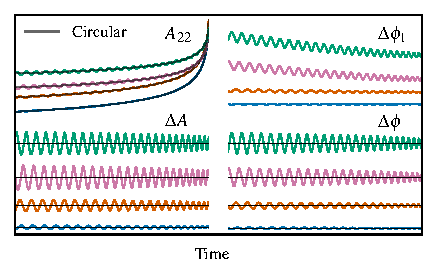
\includegraphics[width=\columnwidth, trim=0.25cm 0.275cm 0.25cm 0.25cm, clip]{Figures/eccentric-residuals.pdf}
    \caption{Amplitude $A_{22}$, eccentric residual amplitude $\Delta A$, residual phase $\Delta \phi_1$, and detrended residual phase $\Delta \phi$ (c.f. Eq. \eqref{eqn: amp-phase-decomp}--\eqref{eqn: residual-circular-phase}) for a few representative $20,000M$ long eccentric \inspiralesigma{} waveforms. Also shown are the amplitudes for the corresponding quasi-circular systems as solid black lines.
    }
    \label{fig: eccentric-residuals}
\end{figure}
%
Finally, we make surrogates for the quasi-circular amplitude $A_{22}(t; \eref=\lref=0, \bm{\theta'})$ and phase $\phi_{22}(t; \eref=\lref=0, \bm{\theta'})$, and for the eccentric residuals $\{\Delta A(t; \param), \Delta \phi(t;\param), \phi_{\rm{res}} (t;\param)\}$. The surrogate model for the eccentric $(2,2)$-mode $h_{22}(t; \param)$ can then be assembled via Eq. \eqref{eqn: residual-amplitude}, \eqref{eqn: residual-phase}, \eqref{eqn: residual-circular-phase} and Eq. \eqref{eqn: amp-phase-decomp}.

\textit{Compressibility of eccentric residuals---} 
Next, we express the training spaces of these data pieces in terms of a few representative basis functions using the greedy basis algorithm \cite{Field:2013cfa}. In Fig.~\ref{fig: surrogate-scaling}, we show the scaling of the number of basis functions required for representing the training space of the eccentric residuals $\Delta A$ and $\Delta \phi$ for different durations of training space waveforms for a fixed (greedy) error threshold of $10^{-5}$~\citep{Field:2013cfa}. 
We observe that a total of $\mathcal{O}(10^{2-3})$ basis functions are required for these contemporary, time-parameterized eccentric residuals. For comparison, a $6.02 \times 10^6M$ long surrogate for quasi-circular waveforms requires only $8$ basis functions in total for $A_{22}$ and $\phi_{22}$ (see Table~\ref{tab: surrogate-metrics}).  This highlights the central issue in eccentric surrogate modeling---the orbital timescale oscillations due to eccentricity in $\Delta A$ and $\Delta \phi$ prevent their efficient compression into a small set of basis functions. It is this issue that we alleviate by parameterizing $\Delta A$ and $\Delta \phi$ in terms of mean anomaly.

%
\begin{figure}
    \centering
    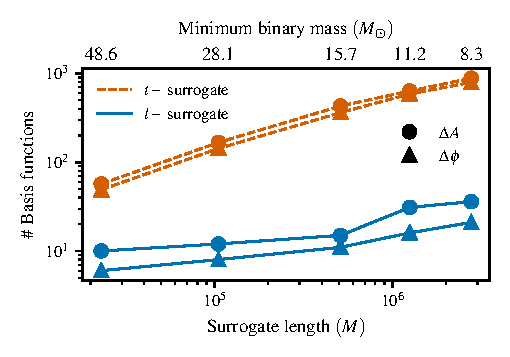
\includegraphics[width=\columnwidth, trim=0.35cm 0.35cm 0.32cm 0.35cm, clip]{Figures/surrogate-scaling.pdf}
    \caption{Number of basis functions required to achieve a greedy error threshold~\citep{Field:2013cfa} of $10^{-5}$ for representing the training spaces of the eccentric residual amplitude $\Delta A$ and phase $\Delta \phi$ for different surrogate lengths for time-parameterized (dashed orange) and mean anomaly parameterized (solid blue) surrogate methodologies. The mean anomaly parameterization achieves the same accuracy with an order of magnitude fewer basis functions. The minimum binary mass for which each surrogate can be evaluated from $15$Hz across its parameter space is indicated at the top, with additional metrics listed in Table~\ref{tab: surrogate-metrics}.}
    \label{fig: surrogate-scaling}
\end{figure}
%

\textit{Novel mean anomaly parameterization---}
$\Delta A$ and $\Delta \phi$ require a relatively large number of basis functions owing to their intricate harmonic content. They oscillate with each periastron and apastron passage of the binary, and the period of these oscillations decreases secularly as the binary inspirals under gravitational radiation reaction, producing the characteristic chirping behavior (see Fig.~\ref{fig: chirp}). Since the chirp rate depends on a binary's eccentricity and mass-ratio, their oscillation period also evolves \textit{differently} across the parameter space. Accurately representing this family of oscillatory functions---whose oscillation periods vary both in time and across parameter space--- therefore requires a large number of basis functions.

Our key idea is to instead model these eccentric residuals against the mean anomaly evolution of the binaries. The mean anomaly evolves via the (orbit-averaged) radial orbital frequency, and thus each radial orbit is separated by $2 \pi$ in mean anomaly for \textit{any} binary configuration, irrespective of eccentricity or mass-ratio. Expressing $\Delta A$ and $\Delta \phi$ against mean anomaly thus eliminates the secular decrease of their oscillation periods (the chirp) over time as well as across the parameter space. The chirp is instead absorbed into the time derivative of the mean anomaly evolution of each binary (see Fig.~\ref{fig: chirp}). Consequently, these \textit{mean anomaly-parameterized eccentric residuals can be represented with an order of magnitude fewer basis functions} than their time-parameterized counterparts (see Fig.~\ref{fig: surrogate-scaling} and Table~\ref{tab: surrogate-metrics}).
%
\begin{figure}
    \centering
    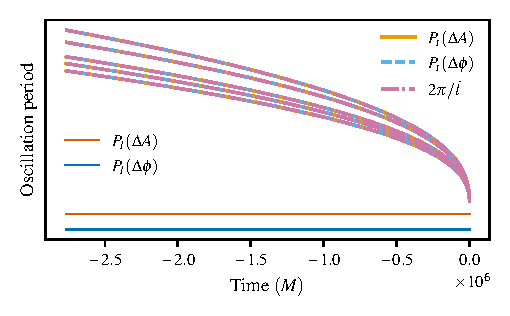
\includegraphics[width=\columnwidth, trim=0.34cm 0.35cm 0.32cm 0.33cm, clip]{Figures/oscillation-periods.pdf}
    \caption{Variation of time/mean-anomaly period of oscillations $P_t(\Delta A)$/$P_l(\Delta A)$ and $P_t(\Delta \phi)$/$P_l(\Delta \phi)$ in $\Delta A$ and $\Delta \phi$ respectively as a function of time for a representative sample of 5 binaries. Their time period of oscillations secularly decreases due to the gradual inspiral of the binary (orange solid and light blue dashed curves), which is the typical chirp of a GW signal. This secular decrease is also encoded in the rate of change of mean anomaly angle of the system (pink dash-dot curve), as evidenced by the mutual overlap of these three sets of curves.
    Therefore, the oscillation period of $\Delta A$ and $\Delta \phi$ in terms of the \textit{mean anomaly} for \textit{any} binary system becomes constant (solid lines; they are vertically offset for visual clarity). In this manner, the chirping behavior of the $\Delta A$ and $\Delta \phi$ oscillations can be factored away into the non-oscillatory time evolution of mean anomaly, simplifying their harmonic content significantly.
    }
    \label{fig: chirp}
\end{figure}

Since all the waveforms end at a constant orbit-averaged orbital frequency at $t=0$, they generally end at different mean anomaly values. For surrogate construction, however, it is necessary to represent the data pieces on a common grid. We therefore model the data-pieces against the \textit{shifted mean anomaly}, $l_s(t; \param) = l(t; \param) - l(t=0; \param)$, so that all the waveforms terminate at $l_s=0$. The shifted mean anomaly, being related to the bare mean anomaly by a constant offset, still has the same time derivative and hence continues to factor away the chirp from the data pieces. We detail the mean anomaly parameterized surrogate construction in Appendix A. 

To get the final waveforms as a function of time, we also need to model the shifted mean anomaly $l_s(t; \param)$ against time. $l_s$ is a monotonically increasing, non-oscillatory function of time (see Fig. \ref{fig: chirp}, which shows its derivative) because it evolves via the \textit{orbit-averaged} radial orbital frequency, and a highly compressed surrogate can be easily built for it. In this work, we get the mean anomaly evolution from the orbital dynamics solver of \inspiralesigma{}. However, it should be possible to work with a definition of mean anomaly that only depends on the waveform morphology~\citep{Shaikh:2023ypz, Shaikh:2025tae}, making this method agnostic to the internal details/conventions of any particular eccentric waveform model; we leave this for future work.   

%===============================================================================

\textit{Simplification of parameter space fits---} Employing the Empirical Interpolation (EI) method~\citep{Field:2013cfa}, we get a set of nodes in time/shifted mean anomaly for each data piece at which fits are constructed for that data piece across the parameter space to yield a continuous surrogate model. We find that for \textit{both} time and mean anomaly parameterized surrogates, the variations in $\Delta A$ and $\Delta \phi$ at these EI nodes is significantly simplified when expressed against the \textit{instantaneous} values of eccentricity and mean anomaly $(e_{EI}, l_{EI})$ at the EI time/shifted mean anomaly nodes, instead of their values $(\eref, \lref)$ at a fixed reference time $t_{\rm{ref}}$ (see Fig.~\ref{fig: parameter-space-variation}). Hence, this simplification allows accurate parametric fits to be built from a relatively sparse training waveform space. We detail the surrogate construction steps in Appendix A. For the same reason, we parameterize the surrogate via the symmetric mass ratio ($\eta:=m_1 m_2/(m_1+m_2)^2$) instead of the mass-ratio $(q)$ for all data pieces.

We use Gaussian Process Regression (GPR) for fitting \cite{Varma:2018aht}. However, we found evaluation of GPR fits to be slow during surrogate evaluation, so we replaced them with faster tensor product cubic spline interpolants~\cite{TPI} constructed over the GPR fit predictions.

%===============================================================================

\textit{Results---} We construct surrogates of increasing waveform durations using both the conventional time-parameterized, as well as our novel mean anomaly-based approach. Their details are summarized in Table~\ref{tab: surrogate-metrics} and Appendix B. The mean anomaly parameterized data pieces require an order of magnitude fewer basis functions, with a gentler scaling of the number of basis functions with surrogate length (c.f. Fig.~\ref{fig: surrogate-scaling}). Also, the mean anomaly parameterized surrogates are more accurate, with their worst mismatches against their base model \inspiralesigma{} being $\mathcal{O}(10^{-5})$ as compared to the time-parameterized surrogates, which exhibit a tail of high mismatches leading to worst mismatches of $10^{-2}-10^{-1}$. These results demonstrate the superior scalability and accuracy of the mean anomaly parameterized approach for constructing long-duration eccentric surrogate models.

Utilizing the scalability of our approach, we construct a $2.77 \times 10^6M$ ($850-1250$ orbits) long eccentric surrogate with a maximum starting eccentricity of $0.43$. Depending on the binary parameters, this time duration corresponds to a $10M_\odot$ binary starting with a GW frequency of $7.2-12$Hz. Figure~\ref{fig: mismatch} shows its mismatches against \inspiralesigma{} for binaries of different masses. The surrogate achieves median mismatches of $1.3-3.2 \times 10^{-6}$, with the worst mismatch of $2.1 \times 10^{-4}$ for a $100M_\odot$ system. Thus, it is faithful to its base model \inspiralesigma{} and can serve as its drop-in replacement within the \esigmahm{} framework~\citep{Paul:2024ujx, esigmapy} for producing full IMR eccentric waveforms (see Fig.~\ref{fig: IMR-surrogate} and Appendix B).   

Fig.~\ref{fig: speedup} shows the waveform generation time for \inspiralesigma{} and the surrogate, and the corresponding speedup achieved. With a starting GW frequency of $15$Hz and a sampling rate of $4096$Hz, the surrogate model is about $20$ times faster to evaluate at its lowest allowed total mass of $8.3M_\odot$, with an evaluation time of about $40$ms, thus making it adequate to analyze such light binary systems using routine LVK Bayesian parameter estimation pipelines.  

\begin{figure}
    \centering
    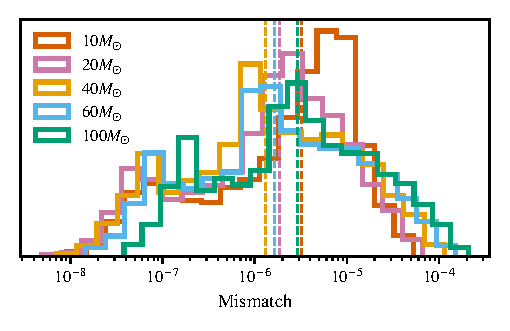
\includegraphics[width=\columnwidth, trim=0.33cm 0.4cm 0.33cm 0.33cm, clip]{Figures/mismatch.pdf}
    \caption{Mismatches of the $2.77 \times 10^6M$ long mean anomaly parameterized surrogate (c.f. Table~\ref{tab: surrogate-metrics}) computed against $10,000$ \inspiralesigma{} waveforms randomly sampled across the surrogate parameter space for binaries of different masses. The mismatches are computed over the full surrogate length, assuming zero-detuning high-power noise power spectral density for the advanced LIGO detector~\citep{LIGO-T0900288-v3, LIGO-T070247-v1}. The dashed lines show the median mismatch values.}
    \label{fig: mismatch}
\end{figure}

\begin{figure}
    \centering
    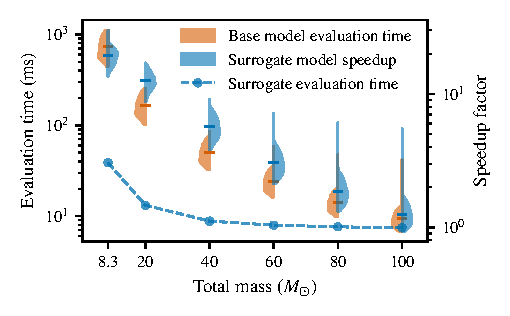
\includegraphics[width=\columnwidth, trim=0.35cm 0.3cm 0.35cm 0.3cm, clip]{Figures/surrogate-speedup.pdf}
    \caption{Waveform evaluation time of the base model \inspiralesigma{} (orange distribution), and the corresponding speedup (blue distribution) and the median evaluation time (blue dots) of its $2.77 \times 10^6M$ long mean anomaly parameterized surrogate for different binary masses. All the waveforms are generated from $15$Hz at a sampling rate of $4096$Hz at 1000 points randomly drawn across the parameter space of the surrogate for each binary mass. The lowest total mass shown corresponds to the smallest value for which the surrogate can be evaluated across its entire parameter space from $15$Hz. Markers also indicate the respective median evaluation times/speedup. The study was performed on an AMD EPYC 7352 processor operating at 2.3 GHz.
    }
    \label{fig: speedup}
\end{figure}

%===============================================================================

\textit{Conclusions---} In this \textit{Letter}, we presented a novel, scalable technique for constructing long-duration eccentric surrogates. The technique aims at simplifying the harmonic content of the eccentricity-induced oscillations in the surrogate data pieces by parameterizing them in terms of the \textit{mean anomaly} angle instead of time, enabling the construction of an order of magnitude more compressed surrogate models than the contemporary time-parameterized methods~\citep{Field:2013cfa, Islam:2021mha}, while being more faithful to the base waveform model. We also significantly simplify the parameter-space fitting of these oscillatory surrogate data pieces by parameterizing them against the \textit{instantaneous} waveform eccentricity and mean anomaly values. 

Leveraging the scalability of the method, we constructed a $2.77\times 10^6M$ ($850-1250$ orbits) long non-spinning, eccentric surrogate of the waveform model \inspiralesigma{}~\citep{Paul:2024ujx} with starting eccentricities up to $0.43$, that can be used to analyze binaries of masses as low as $8.3M_\odot$ from $15$Hz. The surrogate is efficient, taking about $40$ms to evaluate at its full duration, speeding up the waveform generation by an order of magnitude. The scalability of this technique should prove to be useful for constructing eccentric surrogates not only for the current detectors but also for the \textit{future third-generation detectors that will require orders of magnitude longer waveform templates} to observe nearly all the BBH mergers within the era of star formation~\citep{Reitze:2019iox, ET:2019dnz}.

While we have developed surrogates for \inspiralesigma{}, the techniques presented here are general.
In particular, using definitions of eccentricity and mean anomaly based solely on waveform morphology~\citep{Mora:2002gf, Shaikh:2023ypz, Boschini:2024scu, Islam:2025oiv, Shaikh:2025tae} should make this method agnostic to the internal details/conventions of any particular waveform model. Similarly, while our focus was to build long-duration eccentric surrogates, a similar radial phase parameterization has recently enabled accurate short-duration \textit{eccentric numerical relativity surrogate models} \cite{Nee:2025nmh}.

There are some avenues of improvement and additions in this work. The surrogates constructed in this work were restricted to eccentric, non-spinning binaries, and work is ongoing to extend the framework to eccentric, aligned-spin BBH systems. Efforts are also in progress to model sub-dominant higher-order GW modes in addition to the dominant (2,2)-mode.  

Lastly, the operations during surrogate evaluation are highly amenable to parallelization and hardware acceleration (e.g. \cite{Khan:2020fso, Thomas:2022rmc, Thomas:2025rje, Edwards:2023sak}), unlike the ODE-integrated waveform models which are bound to generate waveforms serially. We are also working in this direction to further accelerate waveform generation. 

\begin{acknowledgments}
We would like to thank Md. Arif Shaikh for useful comments on the work. We thank the members of the Astrophysics \& Relativity group at the International Centre for Theoretical Sciences (ICTS) for valuable discussions. A.M. and P.K. acknowledge support of the Department of Atomic Energy, Government of India, under project no. RTI4001 at ICTS. A.M. is an Infosys Fellow supported by the Infosys Foundation and acknowledges the financial support from the Infosys-TIFR Leading Edge travel grant. P.K. acknowledges the support by the Ashok and Gita Vaish Early Career Faculty Fellowship at ICTS.  
CKM acknowledges the support of SERB’s Core Research Grant No. CRG/2022/007959.
V.V.~acknowledges support from NSF Grant No. PHY-2309301.
S.F. acknowledges support from NSF Grants No. AST-2407454 and PHY-2110496.
Parts of this work were carried out during visits to the Institute for Computational and Experimental Research in Mathematics (ICERM) at Brown University; A.M. and P.K. gratefully acknowledge their financial support, with A.M. also acknowledging the support from the International Travel Support (ITS) scheme under the Anusandhan National Research Foundation (ANRF). A.M. also acknowledges the hospitality of the Max Planck Institute for Gravitational Physics (Albert Einstein Institute), Potsdam, where a part of this work was completed.
This work was partly supported by UMass Dartmouth's Marine and Undersea Technology (MUST) research program funded by the Office of Naval Research (ONR) under grant no. N00014-23-1-2141.
All the computations for this work were carried out on the Sonic computing cluster at ICTS. The LIGO document number of this work is LIGO-P2500585. 
\end{acknowledgments}


\bibliography{References.bib}

%===============================================================================
\appendix
\onecolumngrid
\section*{End Matter}
\twocolumngrid

\begin{table*}[]
\caption{Summary of the surrogate models constructed in this work. For each model, we list its length, maximum initial eccentricity ($e_{\rm max}$), number of training points ($N_{\rm train}$), and starting frequency range ($f_0$) for a $10M_\odot$ binary. All the eccentric surrogates are built for mass ratios $\in [1,6]$, while the (time-parameterized) quasi-circular surrogate (last row) is built for mass ratios $\in [1,8]$. We compare the number of basis functions required for the eccentric residuals ($\Delta A, \Delta \phi$) and the median/maximum mismatch against the base model \inspiralesigma{} for both time ($t$) and mean anomaly ($l$) parameterizations.}
\label{tab: surrogate-metrics}
\setlength{\tabcolsep}{5pt}
\begin{tabular*}{\textwidth}{@{\extracolsep{\fill}} c c c c c c c c}
\toprule
\multicolumn{1}{c}{Length} & \multicolumn{1}{c}{$e_{\rm max}$} & \multicolumn{1}{c}{$N_{\rm train}$} & \multicolumn{1}{c}{$f_0$ @ $10 M_\odot$} & \multicolumn{2}{c}{\# Basis functions $(\Delta A, \Delta \phi)$} & \multicolumn{2}{c}{Mismatch @ $10 M_\odot$ (median, max)} \\
\cmidrule(lr){5-6} \cmidrule(lr){7-8}
($10^3 M$) & & & (Hz) & $t$-param. & $l$-param. & $t$-param. & $l$-param. \\
\midrule
23   & 0.067 & 504  & 57--73 & 57, 49   & 10, 6   & $4.9 \times 10^{-6}, 1.0 \times 10^{-2}$ & $2.6 \times 10^{-8}, 9.0 \times 10^{-5}$ \\
105  & 0.11 & 672  & 32--42 & 167, 143 & 12, 8   & $2.4 \times 10^{-4}, 2.6 \times 10^{-1}$ & $6.7 \times 10^{-8}, 3.5 \times 10^{-5}$ \\
510  & 0.21 & 864  & 17--24 & 430, 363 & 15, 11  & ---                            & $1.4 \times 10^{-7}, 1.2 \times 10^{-5}$ \\
1250 & 0.36 & 1152 & 10--17 & 635, 589 & 31, 16  & ---                            & $1.2 \times 10^{-6}, 7.6 \times 10^{-5}$ \\
2770 & 0.43 & 1404 & 7.2--12 & 884, 795 & 36, 21  & ---                            & $3.2 \times 10^{-6}, 5.3 \times 10^{-5}$ \\
\midrule
\multicolumn{8}{c}{Quasi-circular model}\\
\midrule
6020 & 0 & 50 & 7.2--10 & \multicolumn{2}{c}{4, 4 $(A_{22}, \phi_{22})$} & \multicolumn{2}{c}{$1.9 \times 10^{-9}, 3.1 \times 10^{-8}$} \\
\bottomrule
\end{tabular*}
\end{table*}

\textit{Appendix A: Mean anomaly domain surrogate construction steps---}
Collectively denoting the eccentric residuals $\{\Delta A$, $\Delta \phi$, $\phi_{\rm{res}}\}$ by $\bm{f}$, we list the steps of constructing the mean anomaly parameterized surrogate below. 
\begin{enumerate}
    \item Assuming a training set of $N_{\rm{train}}$ inspiral-only waveforms with parameters $\{\param_i\}_{i=1}^{N_{\rm{train}}}$, we extract the \textit{unwrapped} mean anomaly evolution as a function of time $l(t; \param_i)$ from the waveform model's orbital dynamics solver.
    \item We find the mean-anomaly extent of each waveform $\Delta l(\param_i) = l(t=0; \param_i) - l(t=t_0; \param_i)$, where $t_0$ is the starting time of the particular waveform. We then calculate the maximum possible common mean anomaly extent $L$ of the training space waveforms by calculating the minimum of their extents, i.e. $L = \mathrm{min}_i\, \Delta l(\param_i)$. We also denote by $T_L(\param_i)$ the time durations of the waveforms having a mean anomaly extent of $L$. 
    \item We define the \textit{shifted mean anomaly}, 
    \begin{equation}
        l_s(t; \param) = l(t; \param) - l(t=0; \param),
        \label{eqn: shifted mean anomaly}
    \end{equation}
    and model all the eccentric residuals ($\bm{f}$) against it, i.e. as $\bm{f}(l_s; \param_i)$ in $l_s \in [-L, 0]$. We make surrogates $\bm{f_s}(l_s; \param)$ for these data-pieces.
    We set $\phi_{22}(l_s=-L; \param)=\phi_{22}(l_s=-L; \eref=\lref=0, \bm{\theta'})=0$, thus ensuring that $\Delta \phi_1(l_s=-L; \param)=0$ (c.f. Eq. \ref{eqn: residual-phase}).
    \item We also construct a surrogate $l_s^{\rm{sur}}(t; \param)$ of the shifted mean anomaly as a function of time for $t \in [-T_{\rm{min}}^L, 0]$, where $T_{\rm{min}}^L = \mathrm{min}_i \, T_L(\param_i)$ is the maximum possible surrogate length in time for a training space with mean-anomaly extent $L$. Since $l_s$ is a monotonically increasing, non-oscillatory function of time (see Fig. \ref{fig: chirp}), its surrogate requires only a few $(<10)$ basis functions.
    \item Using the shifted mean anomaly surrogate, we can get the surrogates of the eccentric data-pieces as a function of time: $\bm{f_s}(t; \param) = \bm{f_s}(l_s=l_s^{\rm{sur}}(t; \param); \param)$, where $t \in [-T_{\rm{min}}^L, 0]$.
    \item For \textit{both} time-parameterized and mean anomaly-parameterized surrogates, variations in the eccentric residuals $\Delta A$ and $\Delta \phi$ across the parameter space at a particular EI node are significantly simplified when parameterized by the instantaneous values of eccentricity ($e_{\rm{EI}}^k$) and mean anomaly ($l_{\rm{EI}}^k$) at the EI nodes (labeled by the index $k$), instead of their values $(e_{\rm{ref}}, l_{\rm{ref}})$ at a fixed reference time $t_{\rm{ref}}$. This is illustrated in Fig. \ref{fig: parameter-space-variation} for mean anomaly parameterized $\Delta A$ at a shifted mean anomaly EI node. However, in the mean anomaly parameterized case, we find that the parameter space variations in $\phi_{\rm{res}}$ at the shifted mean anomaly EI nodes show oscillations. We found that fixing the eccentric residual phase and the monotonic trend initially to zero, i.e. $\Delta \phi(l_s=-L)=\phi_{\rm{res}}(l_s=-L)=0$ simplifies their structure. This choice still respects the zero starting $(2,2)$-mode phase condition $\Delta \phi_1(l_s=-L; \param)=0$. Hence, we use these initially zeroed-out $\Delta \phi$ and $\phi_{\rm{res}}$ for the mean anomaly parameterized surrogate.
    \item Lastly, we build surrogates of the eccentricity $e(l_s; \param)$ and the (unwrapped) mean anomaly $l(l_s; \param)$ evolution as a function of $l_s$, to evaluate the values of eccentricity ($e_{\rm{EI}}^k$) and (wrapped) mean anomaly ($l_{\rm{EI}}^k$) at the shifted mean anomaly EI nodes $l_s=L_s^k$ at any $\param$ \footnote{Similarly, we build surrogates of the eccentricity $e(t; \param)$ and the (unwrapped) mean anomaly $l(t; \param)$ evolution as a function of $t$ for the time-parameterized surrogates constructed in this work.}. However, since $l_s(t; \param) = l(t; \param) - l(t=0; \param)$, we simply build a parameter space fit for $l(t=0; \param)$ to get the mean anomaly at EI nodes as $l(l_s=L_s^k; \param) = L_s^k + l(t=0; \param)$. 
\end{enumerate}

\begin{figure}
    \centering
    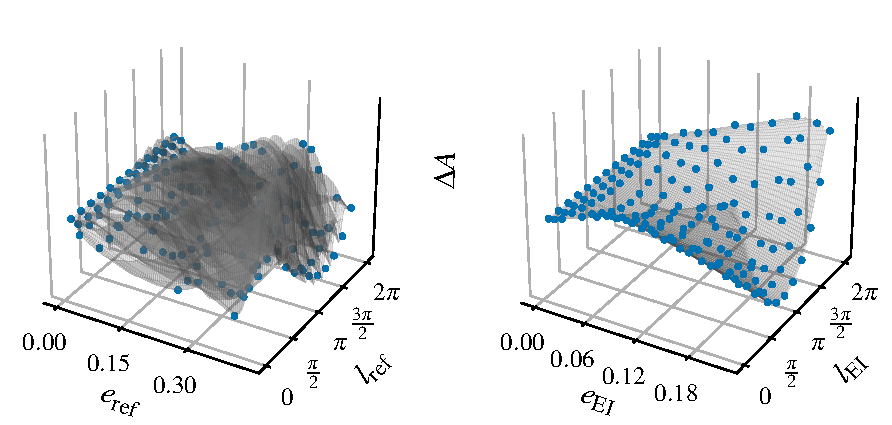
\includegraphics[width=\columnwidth, trim=0.35cm 0.125cm 0.2cm 0.8cm, clip ]{Figures/param-space-variation.pdf}
    \caption{Variation of the eccentric residual amplitude $\Delta A$ at a single empirical interpolation (EI) node across the parameter space for a fixed mass ratio $(q = 3.2)$ for the $2.77 \times 10^6M$ long surrogate. The parameterization in terms of instantaneous values of eccentricity ($e_{\rm{EI}}$) and mean anomaly ($l_{\rm{EI}}$) at the EI nodes (right) yields smoother variation than a parameterization in terms of their values $e_{\rm{ref}}$ and $l_{\rm{ref}}$ at a fixed reference time $t_{\rm{ref}}$ (left). The simplified structure allows for the construction of accurate parametric fits with relatively fewer training space points. $\Delta A$ at a shifted mean anomaly EI node is shown here, and a similar simplification is obtained at time EI nodes as well. 
    }
    \label{fig: parameter-space-variation}
\end{figure}

\begin{figure*}
    \centering
    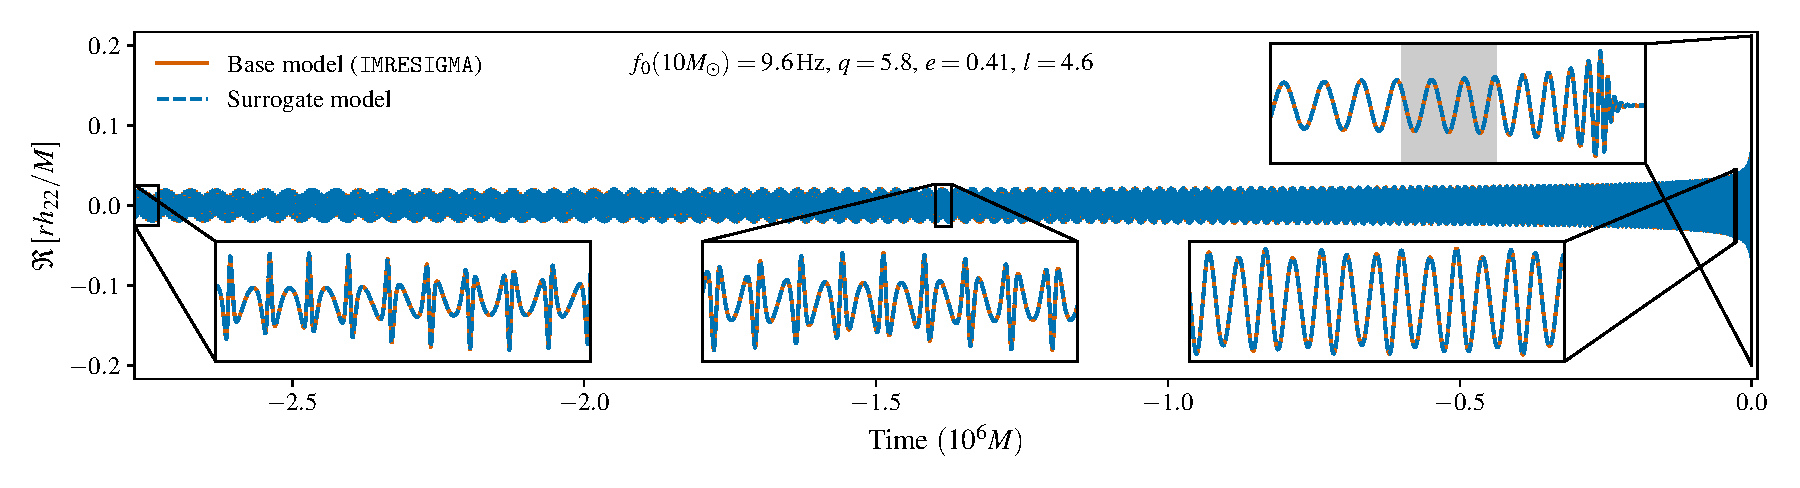
\includegraphics[width=\textwidth, trim=0.54cm 0.53cm 0.53cm 0.52cm, clip]{Figures/IMR-sur-comparison.pdf}
    \caption{The $2.77 \times 10^6M$ long surrogate waveform for \inspiralesigma{} smoothly attached to the plunge-merger-ringdown piece coming from the quasi-circular numerical relativity surrogate \nrsur{} \citep{Varma:2019csw} to produce a hybridized IMR surrogate waveform (blue), and its comparison against \imresigma{} (orange) that employs the same attachment on \inspiralesigma{} \citep{Paul:2024ujx, esigmapy}. The parameters at the start of the waveform are also listed and correspond to the case yielding the worst mismatch ($5.3 \times 10^{-5}$) between the surrogate and \inspiralesigma{} at $10M_\odot$. The surrogate waveform is time and phase shifted by their optimal values found during the match computation.
    The top inset also shows the window (gray band) in which the surrogate is smoothly attached to the plunge-merger-ringdown piece. As highlighted via the insets, the hybridized surrogate waveform remains faithful to the base \imresigma{} waveform from early inspiral through merger-ringdown.} 
    \label{fig: IMR-surrogate}
\end{figure*}

\textit{Appendix B: Summary of all surrogate models---}
To highlight the enhanced scaling and accuracy of the mean anomaly parameterization, we build eccentric, non-spinning surrogates of increasing time durations for the waveform model \inspiralesigma{} using both time and mean anomaly parameterizations. Their metrics are summarized in Table \ref{tab: surrogate-metrics}. 
All the eccentric surrogates cover mass ratios $m_1/m_2\in[1, 6]$, with the maximum starting eccentricity $(e_{\rm{max}})$ chosen such that the eccentricity decays down sufficiently by the end of the inspiral ($e(t=0) \lesssim 0.005$). As required within the \esigmahm{} framework~\citep{Paul:2024ujx, esigmapy}, this allows smooth attachment of a quasi-circular plunge-merger-ringdown piece to construct a hybrid  IMR waveform, as shown in Figure \ref{fig: IMR-surrogate}. Table \ref{tab: surrogate-metrics} also lists the range of minimum starting frequency $f_0$ a $10M_\odot$ binary can be started from and the number of basis functions required to represent the training space of eccentric residuals $\Delta A$ and $\Delta \phi$ within an error threshold of $10^{-5}$ (c.f. Figure \ref{fig: surrogate-scaling}). Only a few basis functions ($\lesssim 10$) are required for the other surrogate data-pieces $\phi_{\rm{res}}(t), \phi_{\rm{res}}(l_s), l_s(t), e(t), e(l_s)$ and $l(t)$ due to their non-oscillatory nature, and are similar in number for both the time and the mean anomaly parameterized approaches and hence are not listed. The median and worst mismatches, computed using the zero-detuning high-power noise power spectral density for the advanced LIGO detector~\citep{LIGO-T0900288-v3, LIGO-T070247-v1} for the full surrogate lengths for a $10M_\odot$ binary against $10,000$ \inspiralesigma{} waveforms randomly sampled across the parameter space of the surrogates, are also listed. We do not proceed beyond basis construction for time-parameterized surrogates longer than $105 \times 10^3M$ because of the large number of basis functions involved, and hence do not have their mismatch data. Lastly, the metrics for the time-parameterized quasi-circular surrogate built for mass ratios $m_1/m_2\in [1,8]$ are also listed, including the number of basis functions required for the quasi-circular amplitude $A_{22}$ and phase $\phi_{22}$. 
The basis construction error thresholds for non-oscillatory data pieces, namely the quasi-circular $A_{22}(t)$ and $\phi_{22}(t)$, and $\phi_{\rm{res}}(t), \phi_{\rm{res}}(l_s), l_s(t), e(t), e(l_s)$ and $l(t)$, are chosen to retain the maximum number of basis functions without noise, as determined through visual inspection.

All the time-domain data pieces are sampled at a uniform spacing of $10M$, except the quasi-circular data pieces at $\simeq 5M$, while the mean anomaly-domain data pieces are sampled uniformly at $2 \pi/100$ (i.e., 100 points per radial orbit). We use linear interpolation over these time/mean anomaly grids to evaluate the surrogates over any user-desired time grid.





\end{document}
